\documentclass[a4paper]{article}

\usepackage{listings}
\usepackage{graphicx}
\usepackage{tabularx}
\usepackage{tikzsymbols}
\usepackage{hyperref}
\usepackage{amsmath}
\usepackage{amssymb}

\usepackage[margin=2cm]{geometry}

\usepackage{titlesec}
\titleformat*{\section}{\large\bfseries}

\definecolor{kit-blue}{RGB}{70, 100, 170}
\input{../slides/l00-commands.tex}

\begin{document}
\exhead{4}{2026-06-16}{2026-06-30}

\newcommand{\statetilled}{T}
\newcommand{\statetobetilled}{$+$}
\newcommand{\statenottobetilled}{$-$}



\section{Variable Elimination ($2 \times 2$ Points)}

Let the formula $S$ with gate encodings $E_1$ and $E_2$ be given.
Apply variable elimination for gates for variables $a$ and $r$.
Give the clause sets after each elimination step.
Try the following two strategies.

\begin{enumerate}\setlength{\itemsep}{1ex}
\item Eliminate variable $a$ first, and then $r$ if possible.
\item Eliminate variable $r$ first, and then $a$ if possible.
\end{enumerate}
\vspace*{-1ex}
\begin{align*}
S = \bigl\{ \underbrace{\{ \lnot x, \lnot y, a \}, \{ x, \lnot a \}, \{ y, \lnot a \}}_{E_1},
\underbrace{\{ \lnot a, r \}, \{ \lnot z, r \}, \{ a, z, \lnot r \}}_{E_2}, \{ a, z, r \},
\{ \lnot a, \lnot r \} \bigr\}
\end{align*}


\section{Variable Elimination with Gate Encodings ($3$ Points)}

For a gate encoding $E$ with output $x$ in a formula $F = E \cup R$,
we simplified the resolvents $(E_x \cup R_x) \otimes (E_{\overline x} \cup R_{\overline x})$ by
$S := (E_x \otimes R_{\overline x}) \cup (R_x \otimes E_{\overline x})$, dropping both
$R_x \otimes R_{\overline x}$ and $E_x \otimes E_{\overline x}$.
Show that the clauses in $R_x \otimes R_{\overline x}$ can be derived from $S$ by resolution.
You can assume that $E$ encodes a binary AND gate.


\section{Blocked Clauses ($3\times 3$ Points)}

If Blocked Clause Elimination (BCE) reduces a formula $F$ to the empty formula then $F$ is called a blocked set.
Prove the following statements.

\begin{enumerate}\setlength{\itemsep}{1ex}
	\item Any formula $F$ can be partitioned into two blocked sets $S$ and $L$ such that $F = S\cup L$.
    Design a linear algorithm that produces $L$ and $S$ from $F$.
	\item Blocked sets are not closed unter resolution. 
    If $F$ is a blocked set then $F \cup C_1 \otimes C_2$, where $C_1,C_2 \in F$ may not be a blocked set anymore.
	\item Blocked sets are not closed unter partially assigning variables.
    If $F$ is a blocked set then $F_{x=v}$ (the result of assigning $v$ to $x$ and subsequent simplification) may not be a blocked set anymore.
\end{enumerate}


\section{Covered Clauses ($3$ Points)}

Let $F$ be a formula and $C \in F$ a clause. 
A literal $l \not\in C$ is called a \emph{covered literal} of $C$ if every non-tautological resolvent of $C$ with a clause in $F$ contains $l$.
The clause $C$ is called \emph{covered} if it becomes blocked in $F$ after adding any of its covered literals.
Prove that adding a covered literal to a clause does not change the satisfiability of the formula.



\section{Competition: SDVSTPP ($10 (+10)$ Points)}
As an extension of the slightly unrealistic SDVSTP (Assignment 2), we introduce the much more precise \emph{Stardew Valley Soil Tilling Planning Problem} (SDVSTPP).
The difference between SDVSTP and SDVSTPP is that the latter now features discrete \emph{time steps} as well as a \emph{player}.
At any given point in time, the player is positioned at exactly one of the grid cells.
At each time step, the player performs one out of two possible kinds of actions:

\begin{enumerate}\setlength{\itemsep}{1ex}
\item \emph{walk} to one of the up to four adjacent tiles,
\item perform some tilling action at one of the up to four adjacent tiles.
\end{enumerate}

\noindent
The tilling action's orientation is decided by the player position.
Figure~\ref{fig:sdvstp-player} shows all potentially valid operations for each of the five patterns, where the black square is the player's location.\\[1em]

\begin{figure}[ht]
	\centering
	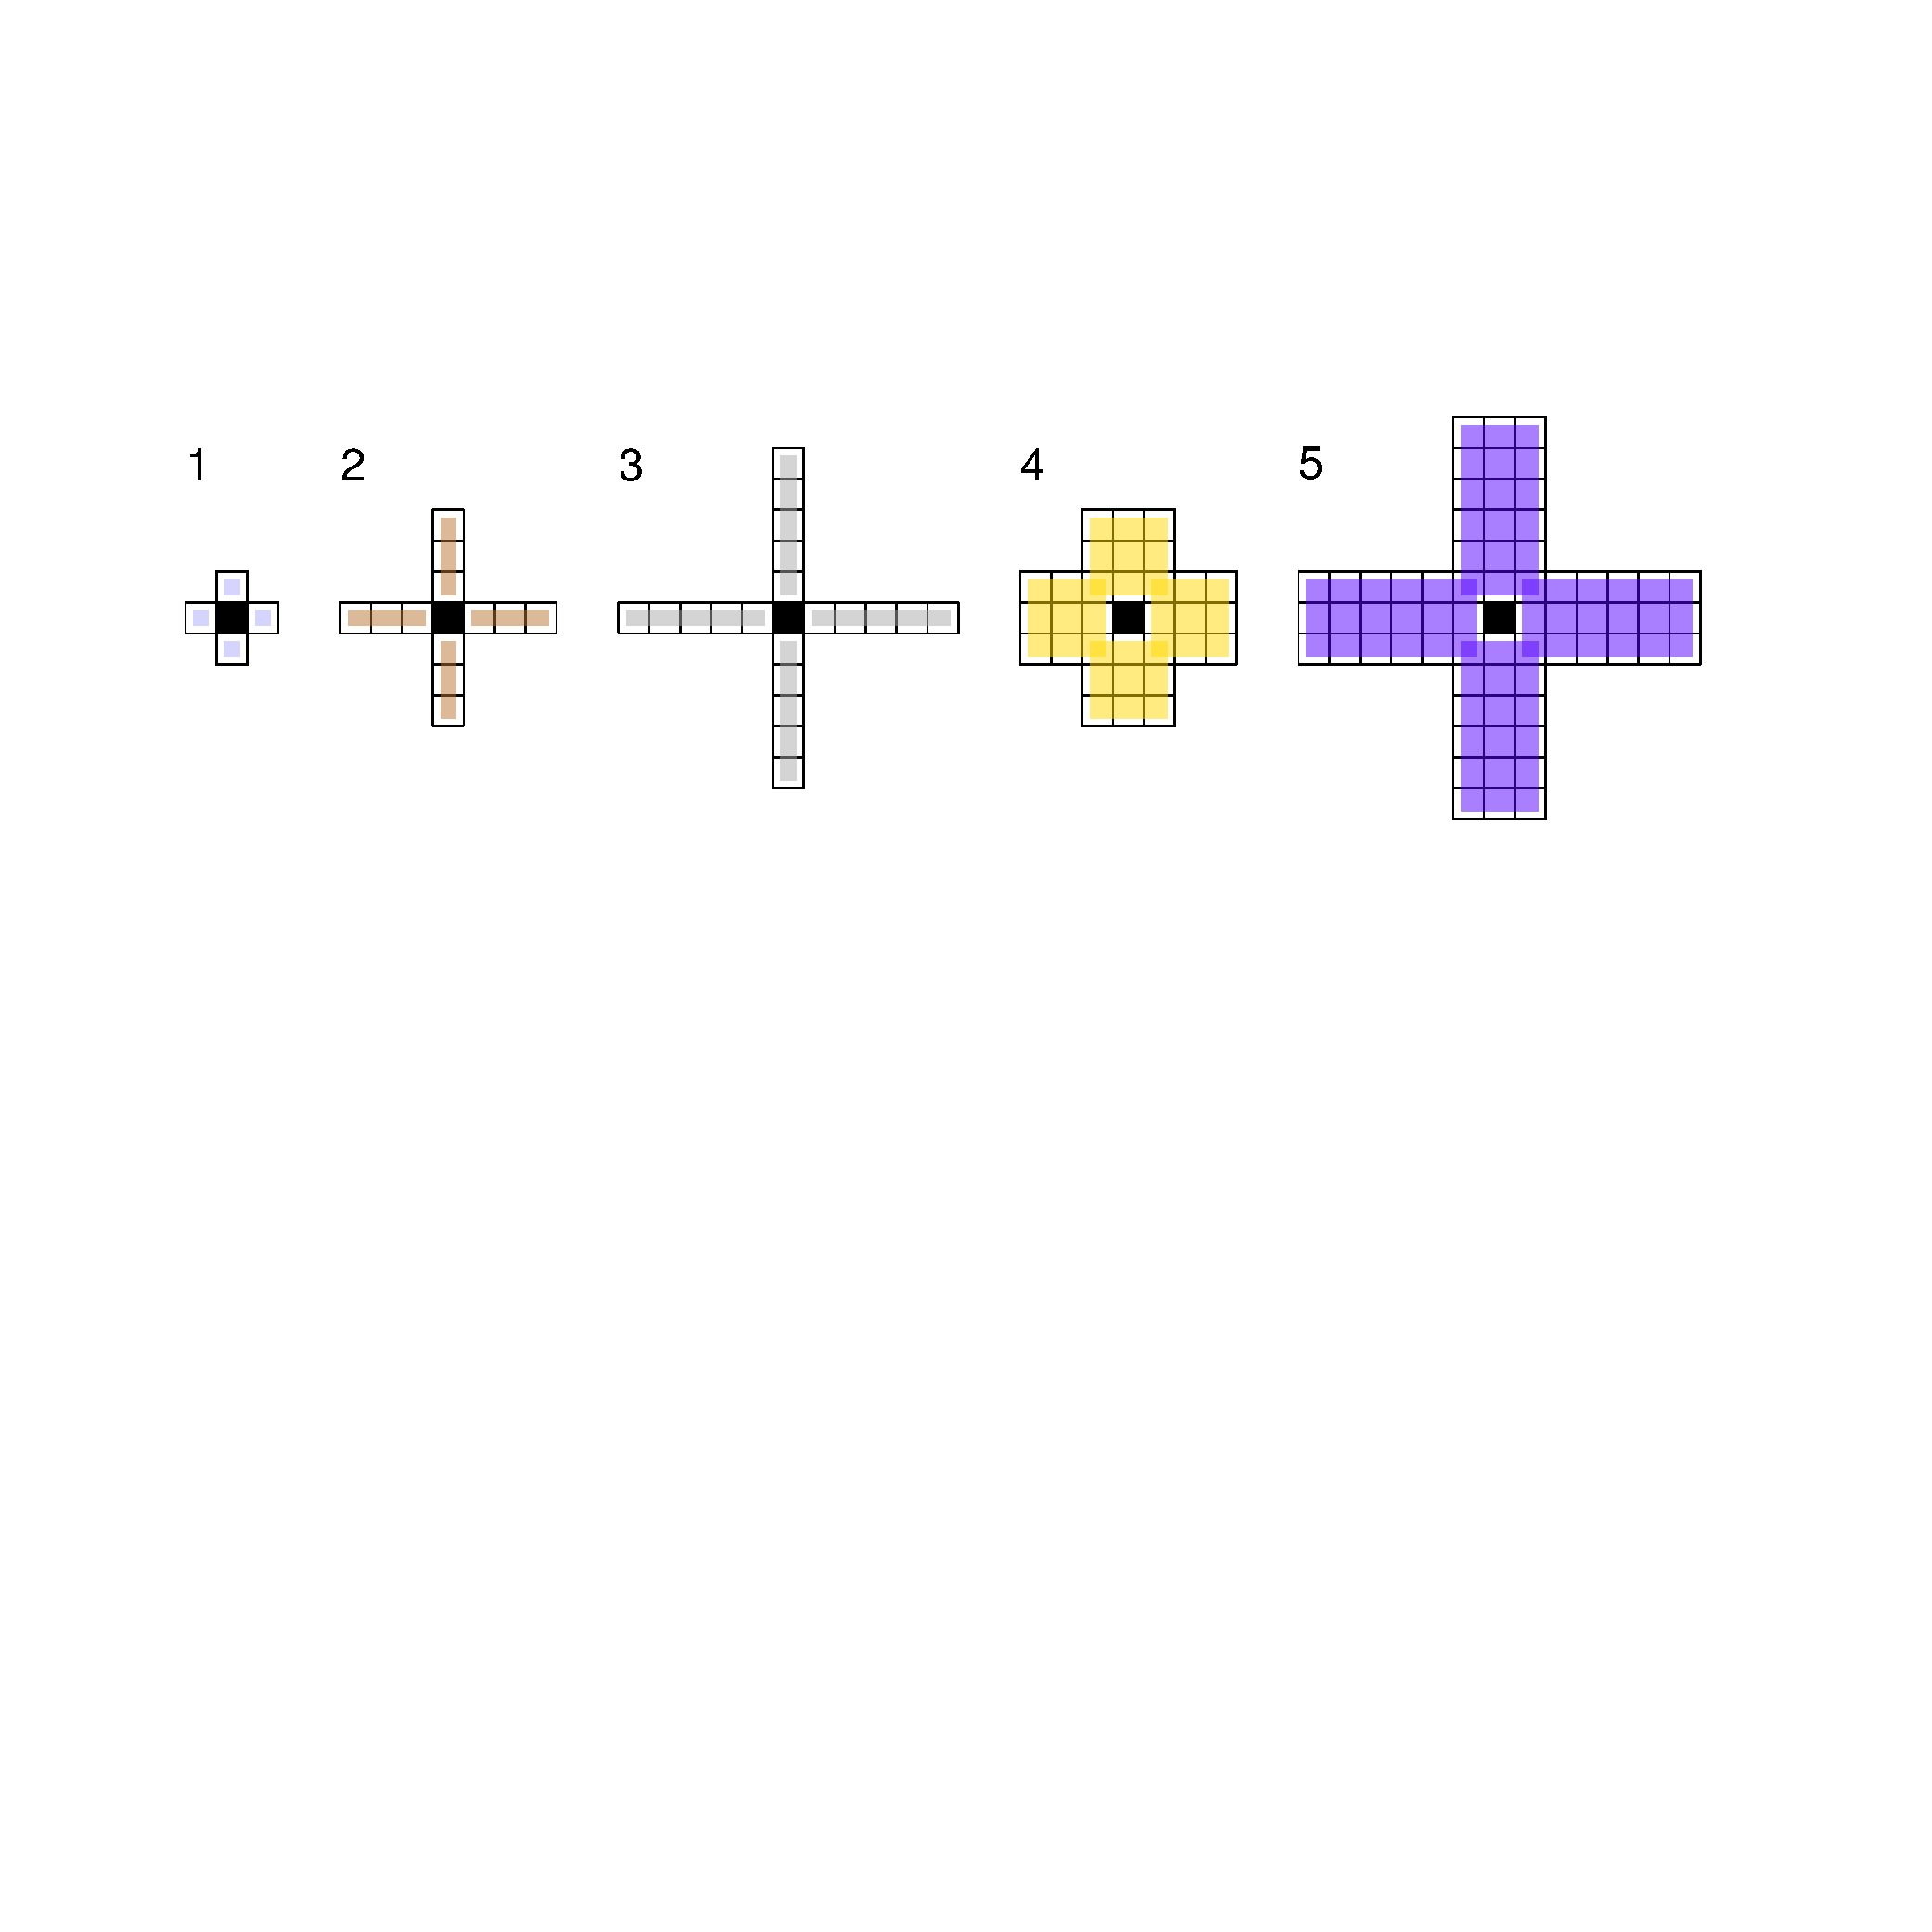
\includegraphics[width=11cm]{figures/sdvstp-player.pdf}
	\caption{The five tilling patterns and their valid orientations.}
	\label{fig:sdvstp-player}
\end{figure}

\noindent
Your task is to write an \textit{optimal SAT-based SDVSTPP planner}.
The planner application takes an \texttt{.sdvstp} file (just like the SDVSTP solver in Assignment 2) and assumes that the player is initially located at the \emph{top left position}, i.e., at the first cell character read from the \texttt{.sdvstp} file.
The planner should output the shortest possible plan in terms of time steps (i.e., player actions) that results in a grid state where tiles are tilled exactly according to the input specification (as in SDVSTP).\\[1em]

\noindent
As shown in Figure~\ref{fig:sdvstpp-solution}, the plan should be output as a single line beginning with ``\texttt{s }'', where \texttt{U}/\texttt{D}/\texttt{L}/\texttt{R} corresponds to up/down/left/right movement and where \texttt{u}/\texttt{d}/\texttt{l}/\texttt{r} followed by \texttt{1}/\texttt{2}/\texttt{3}/\texttt{4}/\texttt{5} corresponds to tilling action 1--5 in up/down/left/right direction, respectively.

\begin{figure}[ht]
	\centering
	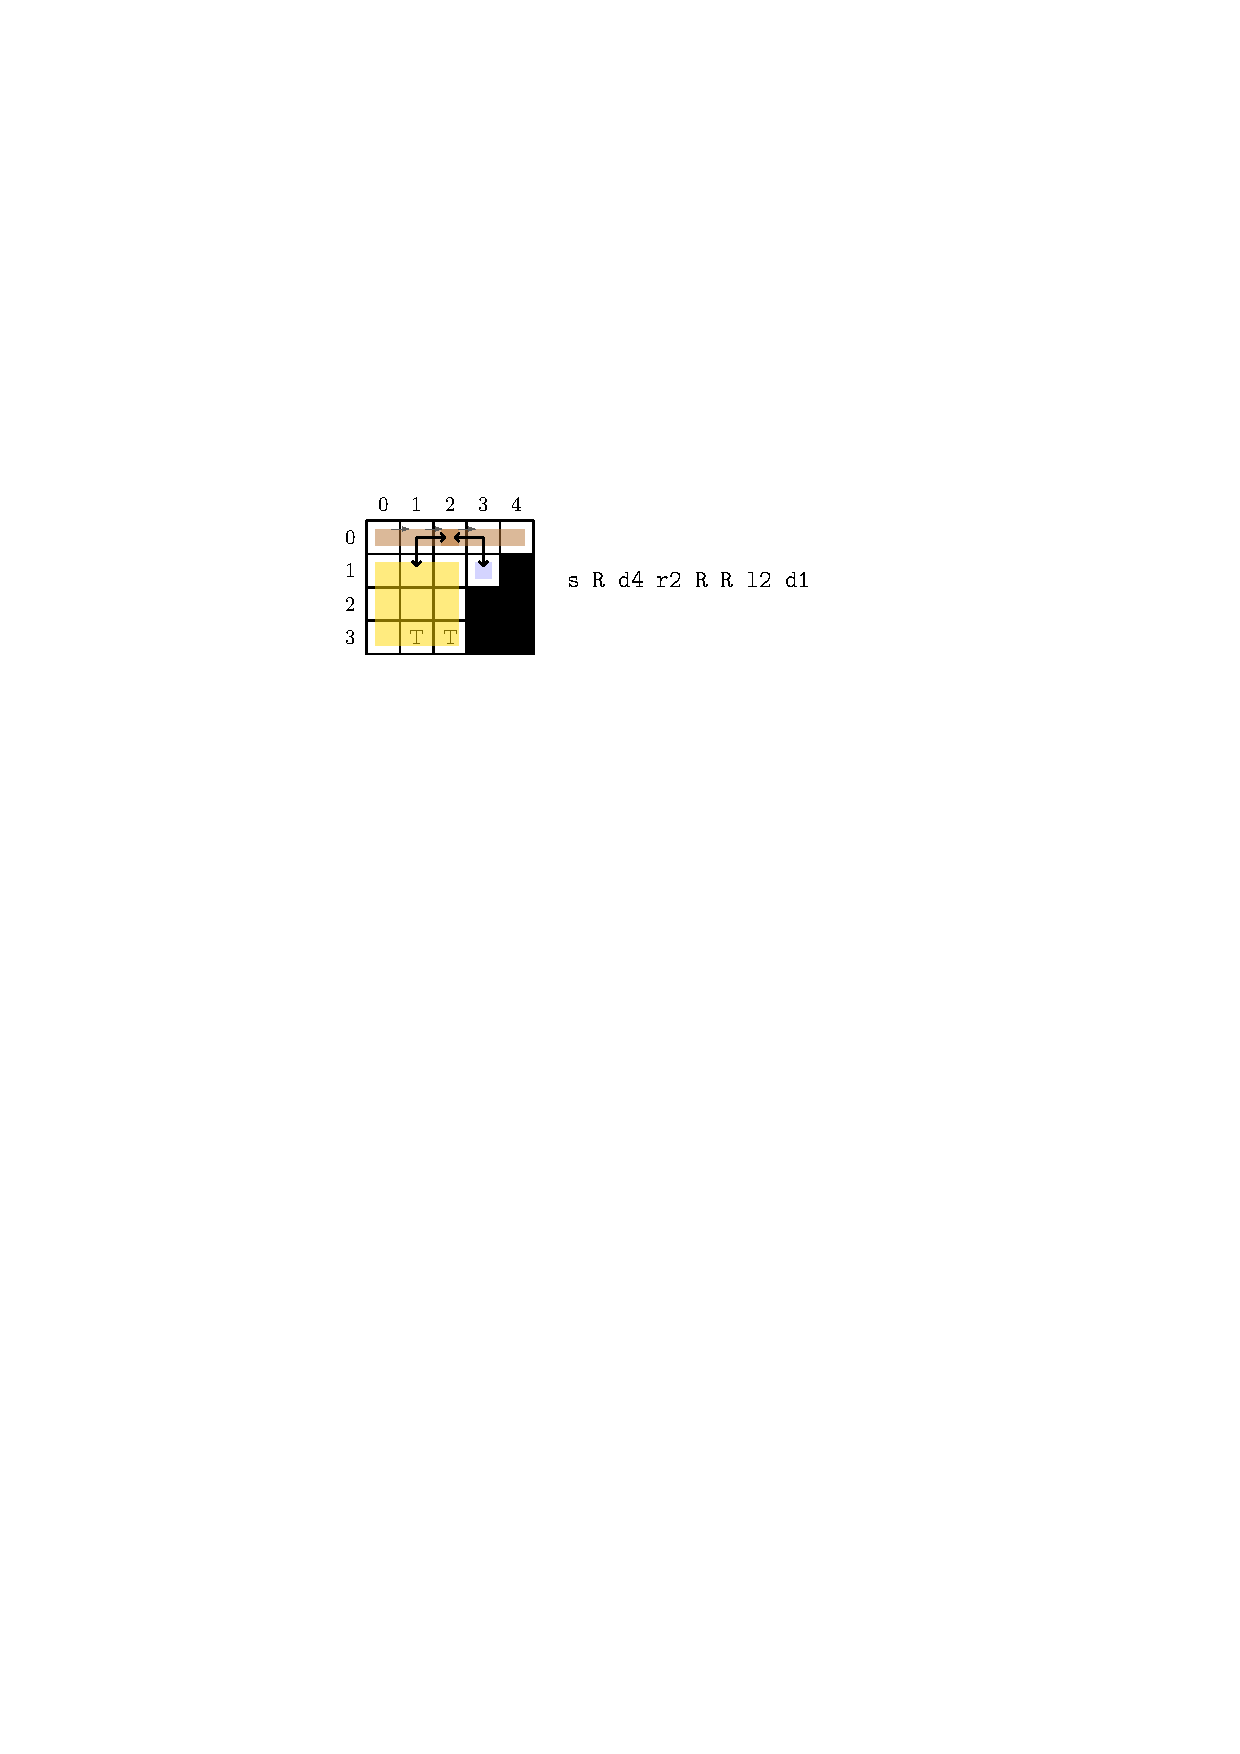
\includegraphics[width=6.5cm]{figures/sdvstpp-solution.pdf}
	\caption{An example of an optimal SDVSTPP plan.}
	\label{fig:sdvstpp-solution}
\end{figure}

\noindent
You receive 10 points for an optimal planner solving easy inputs and up to 10 bonus points for solving more difficult inputs.

\vspace*{3mm}
\noindent
\textbf{Code skeleton:} \url{https://github.com/satlecture/kit2025/blob/main/code/src/sdvstp/sdvstpp.cc}
\\[1ex]
\noindent
\textbf{Some benchmark instances:} \url{https://github.com/satlecture/kit2025/tree/main/exercises/sdvstp}


\end{document}